\chapter{Results Analysis}
\label{chap:results}

This chapter reports the results of every task in the order of the problem statement, then discusses them. All numbers are measured on test data that were not used for training or model selection.

\section{Experimental Setup}

Review-level models are evaluated on the test sets of scenario A (1,496 reviews of known games) and scenario B (1,955 reviews of 20 unseen games) described in Section~\ref{sec:splits}, with ROC-AUC as the main metric and accuracy at a threshold of 0.5 as a secondary one. Aspect-level models are evaluated on the labelled sentence sets, with Test 2 as the main set. Transformer results are averaged over seeds, and a difference is considered reliable when its 95\% paired-bootstrap CI does not contain zero.

\section{Task 1: Review Sentiment Classification}

\begin{table}[!htbp]
\centering
\caption{Sentiment classification on the test sets of scenario A (known games) and B (unseen games)}
\label{tab:sentiment}
\begin{tabular}{lcccc}
\toprule
\multirow{2}{*}{\textbf{Model}} & \multicolumn{2}{c}{\textbf{Accuracy}} & \multicolumn{2}{c}{\textbf{ROC-AUC}} \\
\cmidrule(lr){2-3}\cmidrule(lr){4-5}
 & A & B & A & B \\
\midrule
Meta features only + LR & 0.661 & 0.657 & 0.716 & 0.711 \\
TF-IDF + LR & 0.818 & 0.827 & 0.903 & 0.906 \\
TF-IDF + meta + LR & 0.825 & 0.836 & 0.908 & 0.909 \\
\midrule
M1 Embedding + Pooling & 0.741 & 0.801 & 0.836 & 0.883 \\
M2 BiLSTM & 0.801 & 0.799 & 0.884 & 0.893 \\
M3 CNN 1D & 0.797 & 0.794 & 0.871 & 0.883 \\
M4 TF-IDF + Dense & 0.812 & 0.815 & 0.891 & 0.893 \\
M5 Ensemble (M2 + M4) & 0.824 & 0.826 & 0.902 & 0.905 \\
\midrule
DistilBERT (mean of 3 seeds) & $\approx$0.86 & $\approx$0.855 & \textbf{0.937} & \textbf{0.930} \\
\bottomrule
\end{tabular}
\end{table}

Table~\ref{tab:sentiment} leads to four observations:
\begin{itemize}
    \item \textbf{The text carries most of the information.} Meta features alone reach a ROC-AUC of about 0.71, TF-IDF + LR on the text 0.90; adding meta features to TF-IDF adds only 0.005.
    \item \textbf{Keras models trained from scratch do not beat TF-IDF + LR.} With fewer than 7,000 training reviews, M1--M3 start to overfit after 2--3 epochs. M4 is the best single Keras model, and the ensemble M5 matches the LR baseline (0.902 versus 0.903 in scenario A).
    \item \textbf{The models generalise to unseen games}: scores in scenario B are not lower than in scenario A, so the models learn general ways of praising and complaining rather than game-specific words.
    \item \textbf{DistilBERT is the best model}, with a ROC-AUC of 0.937 (A) and 0.930 (B). The 95\% CI of its gain over TF-IDF + LR is $[+0.026, +0.047]$ in scenario A and $[+0.017, +0.037]$ in scenario B, well above the variation between seeds (about 0.002).
\end{itemize}

\textbf{Error analysis.} M4 misses mild complaints more often than praise: on test set A, 25\% of negative reviews are classified as positive but only 13\% of positive reviews as negative, and accuracy drops from about 85\% for reviews longer than 50 words to 73\% for reviews of at most five words. The 500 manually labelled reviews show where the remaining difficulty lies (Table~\ref{tab:erroranalysis}). Both models are very accurate on clear reviews; jokes, mixed and unclear reviews are much harder. Reading the errors, DistilBERT reduces genuine model errors from 46 to 26, while errors caused by a Steam verdict that contradicts the text stay almost constant (13 and 14). No model can fix those, and they are exactly what Task 2 tries to find. Sarcasm such as ``Oh great, another update that breaks everything. Love it.'' is still read as positive by M4.

\begin{table}[!htbp]
\centering
\caption{ROC-AUC on the 500 manually labelled test reviews}
\label{tab:erroranalysis}
\begin{tabular}{lrcc}
\toprule
\textbf{Group of reviews} & \textbf{Reviews} & \textbf{M4} & \textbf{DistilBERT} \\
\midrule
All & 500 & 0.887 & 0.931 \\
Clear sentiment, normal reviews & 365 & 0.942 & 0.968 \\
Others (jokes, mixed, unclear, \ldots) & 135 & 0.672 & 0.758 \\
\bottomrule
\end{tabular}
\end{table}

\section{Task 2: Suspicious Review Detection}

The out-of-fold M4 predictions reach an accuracy of 0.82 and a ROC-AUC of 0.90, the same level as on the held-out test set, so they can serve as a measure of what the text says. Table~\ref{tab:suspicious} and Figure~\ref{fig:suspicious} summarise the result of Algorithm~\ref{alg:suspicious}.

\begin{table}[!htbp]
\centering
\caption{Suspicious reviews among the 9,971 cleaned reviews}
\label{tab:suspicious}
\begin{tabular}{lrr}
\toprule
\textbf{Criterion} & \textbf{Reviews} & \textbf{\%} \\
\midrule
Quality rules (any flag) & 20 & 0.20 \\
Content--verdict mismatch & 270 & 2.71 \\
\quad Negative text but recommended & 170 & 1.70 \\
\quad Positive text but not recommended & 100 & 1.00 \\
\midrule
\textbf{Suspicious (rules or mismatch)} & \textbf{290} & \textbf{2.91} \\
Uncertain model ($|p - 0.5| < 0.1$), reported separately & 1,078 & 10.81 \\
\bottomrule
\end{tabular}
\end{table}

\begin{figure}[!htbp]
    \centering
    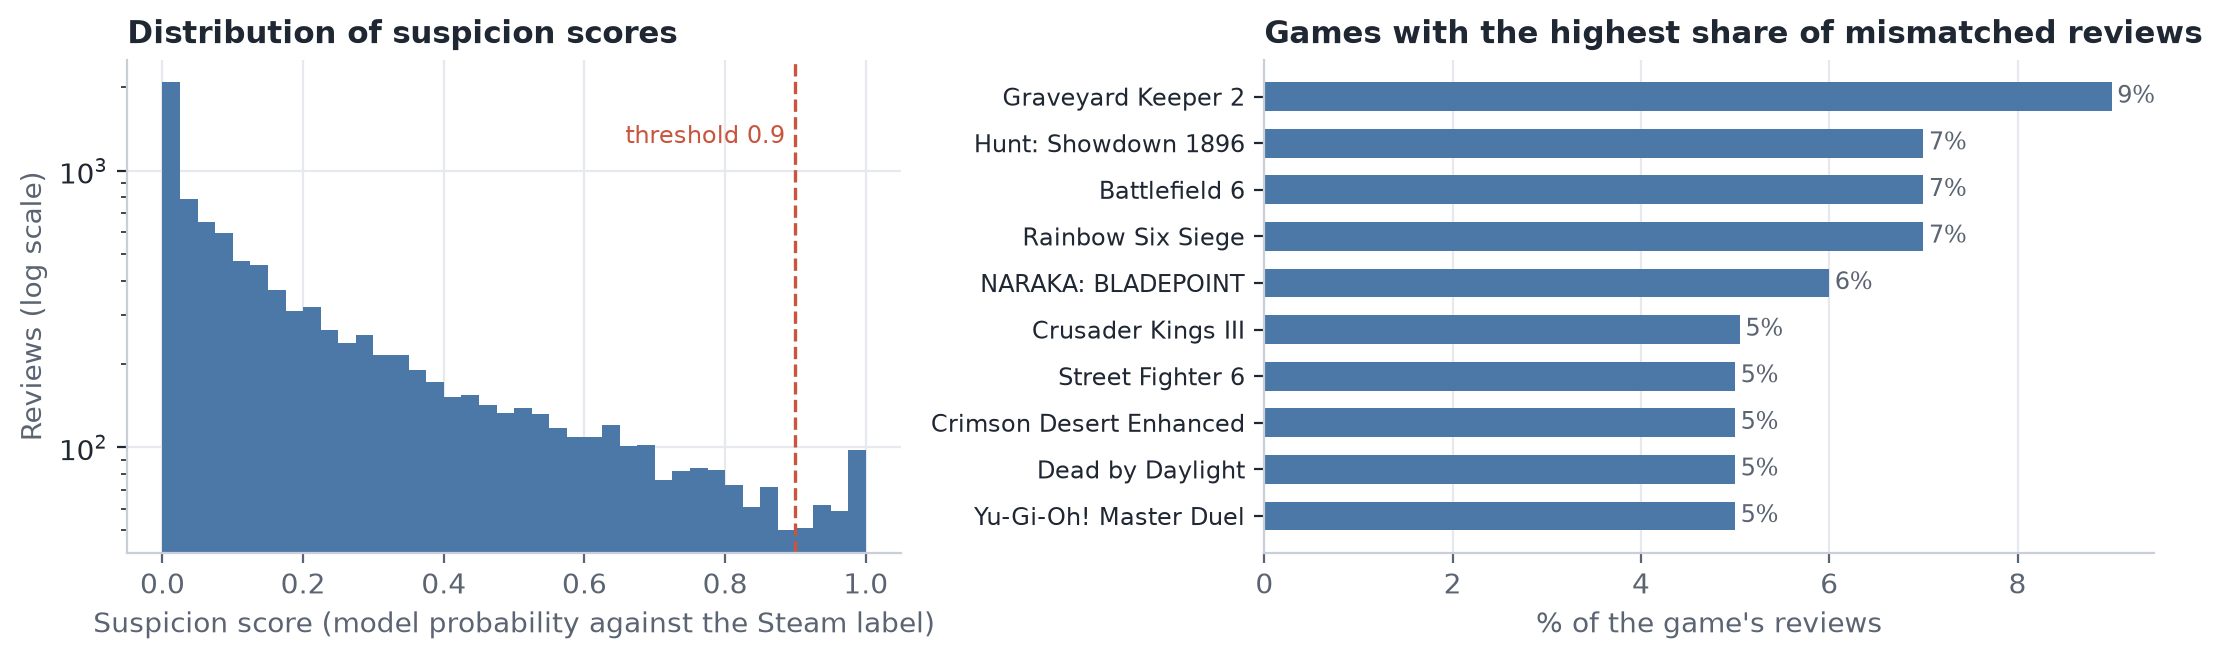
\includegraphics[width=0.95\textwidth]{fig13_suspicious.png}
    \caption{Distribution of suspicion scores (log scale) and games with the highest share of mismatched reviews.}
    \label{fig:suspicious}
\end{figure}

The quality rules catch only 20 reviews, so the cleaned data contain little obvious spam; the mismatch criterion is more informative. Reading the flagged reviews reveals three groups: \textbf{sarcasm and trolling} (``10/10 would never play again'', not recommended), \textbf{mixed reviews} that list strengths but conclude ``I can't recommend it'' or list bugs and still recommend, and \textbf{probable misclicks} with entirely positive text and a negative verdict. Several competitive online games are among those with the most mismatched reviews, but even for them the share stays below 10\%. Without ground-truth labels the precision of the flags cannot be computed, so the output is meant as a ranked list for human moderators rather than an automatic filter.

\section{Task 3: Helpfulness Prediction}

\begin{table}[!htbp]
\centering
\caption{Predicting whether a review receives at least one helpful vote (test set A)}
\label{tab:helpful}
\begin{tabular}{lccc}
\toprule
\textbf{Model} & \textbf{F1} & \textbf{ROC-AUC} & \textbf{PR-AUC} \\
\midrule
LR, review age only & 0.065 & 0.624 & 0.429 \\
LR, meta features + age & 0.515 & 0.771 & 0.601 \\
TF-IDF + meta + age, LR & 0.542 & \textbf{0.786} & \textbf{0.636} \\
Keras M4 + meta + age (class weights) & \textbf{0.611} & 0.761 & 0.605 \\
\bottomrule
\end{tabular}
\end{table}

Review age alone gives a ROC-AUC of 0.62, which confirms that it must be controlled for (Table~\ref{tab:helpful}). Meta features raise it to 0.77 and the text to 0.79, so content and length help beyond age. Keras M4 has a slightly lower ROC-AUC but the best F1 (0.61) thanks to class weighting. The strongest factor is the sentiment label: 51.9\% of negative reviews have a helpful vote against 13.2\% of positive ones, followed by review length. Because negative reviews in this dataset are also older, part of this effect comes from the sampling.

\section{Task 4: Aspect-Based Sentiment Analysis}

\subsection{Aspect Detection}

\begin{table}[!htbp]
\centering
\caption{Aspect detection (micro F1, mean over seeds). The variant selected on dev is in bold.}
\label{tab:aspectdet}
\begin{tabular}{lrccc}
\toprule
\textbf{Method} & \textbf{Train sentences} & \textbf{Dev} & \textbf{Test 2} & \textbf{Test 1} \\
\midrule
Keywords & 0 & 0.546 & 0.557 & 0.640 \\
TF-IDF + LR & 2,913 & 0.605 & 0.602 & 0.602 \\
DistilBERT & 1,265 & 0.655 & 0.606 & 0.635 \\
Keywords-in-input & 1,265 & 0.692 & 0.640 & 0.696 \\
Keywords-in-input & 1,995 & 0.708 & 0.665 & 0.714 \\
\textbf{Keywords-in-input} & \textbf{2,725} & \textbf{0.733} & \textbf{0.682} & \textbf{0.722} \\
Keywords-in-input & 2,913 & 0.731 & 0.692 & 0.731 \\
DistilBERT & 2,913 & 0.729 & 0.679 & 0.715 \\
Union of keywords and DistilBERT & 2,913 & 0.722 & 0.687 & 0.723 \\
\bottomrule
\end{tabular}
\end{table}

Table~\ref{tab:aspectdet} shows that:
\begin{itemize}
    \item \textbf{The transformer clearly beats keywords and TF-IDF.} On Test 2 the selected model is 0.125 above the keywords (CI $[0.085, 0.169]$) and 0.080 above TF-IDF + LR (CI $[0.040, 0.120]$).
    \item \textbf{Keyword hints help most when labels are scarce:} +0.033 over plain DistilBERT with 1,265 sentences, but only +0.003 with about 2,900 sentences, where the CI contains zero ($[-0.017, 0.024]$).
    \item \textbf{More labels help with diminishing returns}: +0.025, then +0.017 per additional 730 sentences.
    \item \textbf{Keywords alone have low recall} (precision 0.735, recall 0.448 on Test 2). Their higher score on Test 1 (0.640) reflects that they were written after reading that set, which justifies Test 2 as the main test set.
\end{itemize}
Per aspect, gameplay gains most over keywords (F1 0.47 to 0.71), because players describe gameplay in many ways that are hard to list. Online/community and developer remain harder (0.64 and 0.68), and audio (3 test sentences) and graphics (21) have too few examples for reliable conclusions.

\subsection{Aspect Polarity}

On the 765 (sentence, aspect) pairs with a positive or negative gold label, the pairwise model reaches an accuracy of 0.898, against 0.689 for always predicting ``negative'' (Table~\ref{tab:polarity}).

\begin{table}[!htbp]
\centering
\caption{Aspect polarity accuracy compared with whole-sentence models}
\label{tab:polarity}
\begin{tabular}{lccc}
\toprule
\textbf{Whole-sentence baseline} & \textbf{Accuracy} & \textbf{Pairwise gain} & \textbf{95\% CI} \\
\midrule
M4 & 0.742 & +0.156 & $[+0.125, +0.188]$ \\
DistilBERT & 0.835 & +0.063 & $[+0.042, +0.085]$ \\
\bottomrule
\end{tabular}
\end{table}

Two weaknesses remain. First, \textbf{sentences with conflicting aspects are not solved}: on the 55 pairs from sentences that praise one aspect and criticise another, all three models reach about 0.55 (ROC-AUC 0.58 for the pairwise model), and adding 188 such sentences to training changed nothing (0.552 versus 0.545). This was the case the pairwise formulation was meant to solve, so this objective was not met, although with 55 pairs the CI is wide ($[-0.145, +0.139]$ against M4). Second, \textbf{the model leans towards negative}: compared with M4, accuracy on negative pairs rises from 0.674 to 0.930, but on positive pairs it drops from 0.895 to 0.826.

\subsection{End-to-End Pipeline and Results per Game}

\begin{table}[!htbp]
\centering
\caption{End-to-end aspect sentiment pipeline (a pair is correct only if both aspect and polarity are correct)}
\label{tab:pipeline}
\begin{tabular}{lcccc}
\toprule
\multirow{2}{*}{\textbf{Pipeline}} & \multicolumn{3}{c}{\textbf{Test 2}} & \textbf{Test 1} \\
\cmidrule(lr){2-4}\cmidrule(lr){5-5}
 & P & R & F1 & F1 \\
\midrule
Keywords + M4 (first version) & 0.572 & 0.372 & 0.451 & 0.494 \\
Keywords + whole-sentence DistilBERT & 0.611 & 0.397 & 0.481 & 0.549 \\
Keywords + pairwise DistilBERT & 0.638 & 0.414 & 0.502 & 0.579 \\
\textbf{Keywords-in-input + pairwise DistilBERT} & 0.607 & \textbf{0.638} & \textbf{0.622} & \textbf{0.640} \\
\bottomrule
\end{tabular}
\end{table}

The end-to-end F1 rises from 0.451 to 0.622 (Table~\ref{tab:pipeline}), almost entirely through recall (0.372 to 0.638) while precision stays similar: the final pipeline finds many more aspect opinions without proportionally more mistakes. Both test sets rank the four pipelines in the same order.

Applied to all 33,025 sentences of the 99 games, the pipeline produced 24,223 (aspect, polarity) pairs; since some sentences were used in training, this is a description rather than an evaluation. Gameplay is by far the most discussed aspect (10,297 mentions). Players are most negative about performance and bugs (90.3\% of mentions) and developers (85.2\%), and least about graphics (31.0\%) and audio (43.7\%). Figure~\ref{fig:aspectgame} shows clear differences between games, the kind of summary a developer could use to prioritise fixes. The percentages should only be compared relatively, because of the 50/50 sampling per game, the longer negative reviews, the negative lean of the polarity model and the small number of sentences in some cells.

\begin{figure}[!htbp]
    \centering
    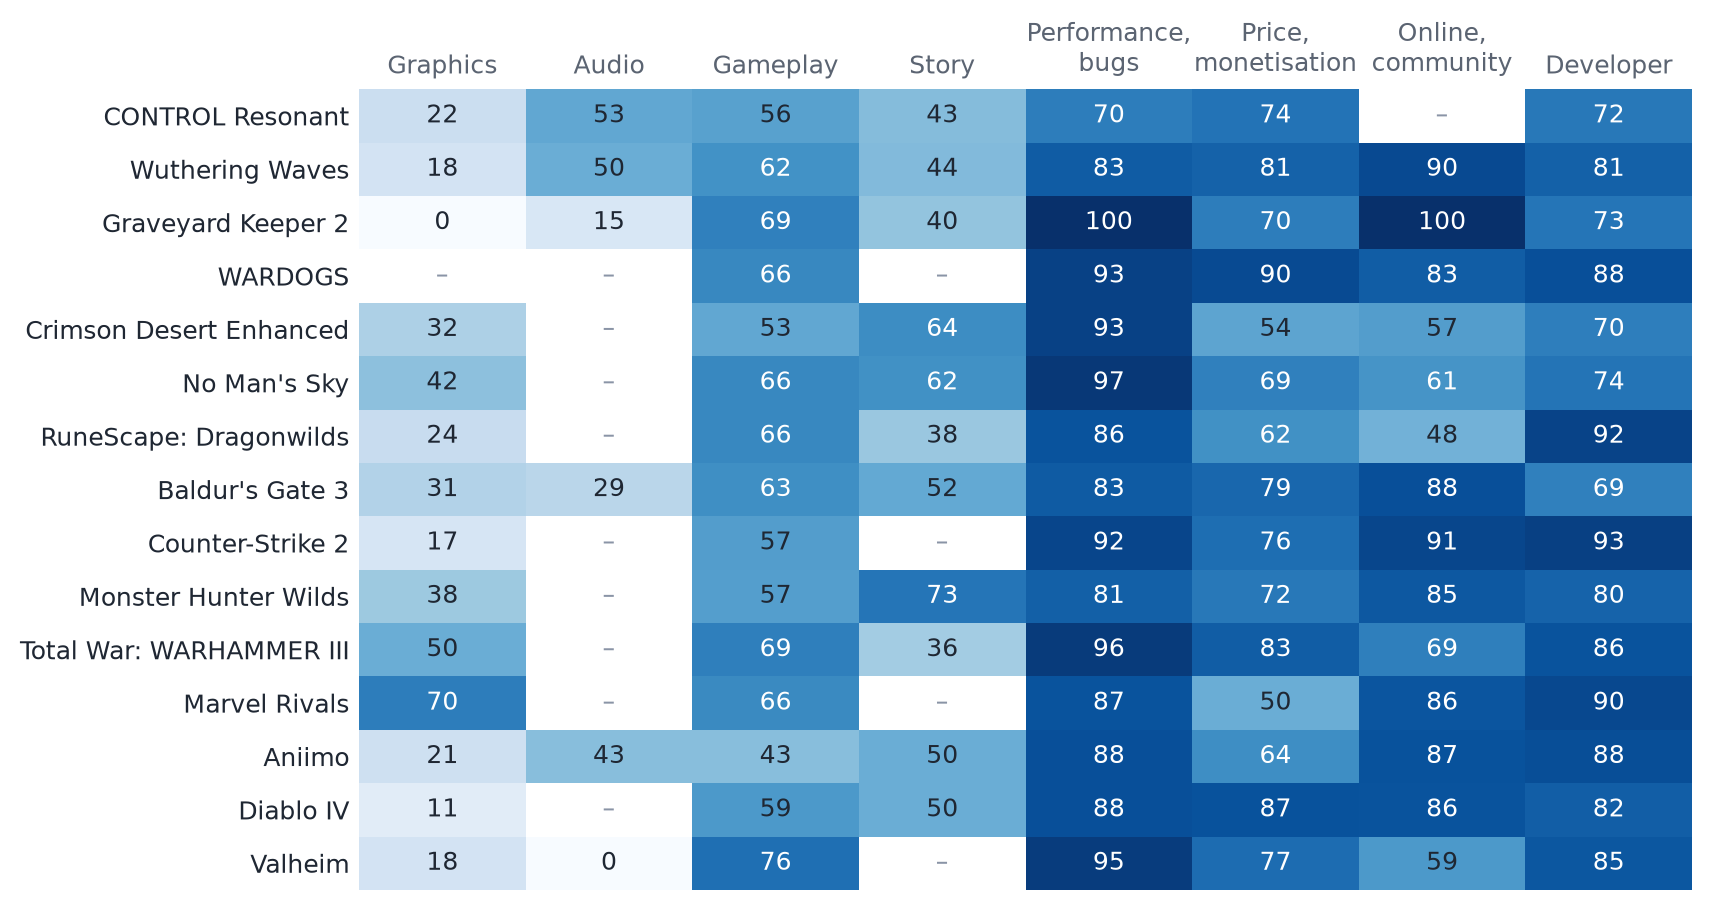
\includegraphics[width=0.75\textwidth]{fig10_aspect_by_game.png}
    \caption{Share of negative sentences (\%) per aspect for the 15 games with the most sentences; ``--'' marks fewer than 5 sentences.}
    \label{fig:aspectgame}
\end{figure}

\section{Task 5: Game Recommendation and Demo Application}

Figure~\ref{fig:appreco} shows the recommendation page of the demo application for a user who liked \textit{Stardew Valley}. Its genre is ``Life \& Job Sim'' and its publisher has no other game in the data, so all candidates share the genre and are ranked by their positive rating (Euro Truck Simulator 2, Slime Rancher and Dave the Diver at 97\%, then Slime Rancher 2 and Supermarket Simulator). The graph groups games around genre and publisher nodes, as suggested by the instructor. Because each user has a single review and there is no record of what users played next, the recommendations cannot be evaluated quantitatively; the result demonstrates the method. The other pages of the application apply the Task 1--3 models: for example, a clearly positive review submitted as ``Not recommended'' receives a positive probability of 99\% and is flagged as suspicious, and the batch page summarises all reviews of a game with the share of negative reviews by playtime and the most frequent words in negative reviews.

\begin{figure}[!htbp]
    \centering
    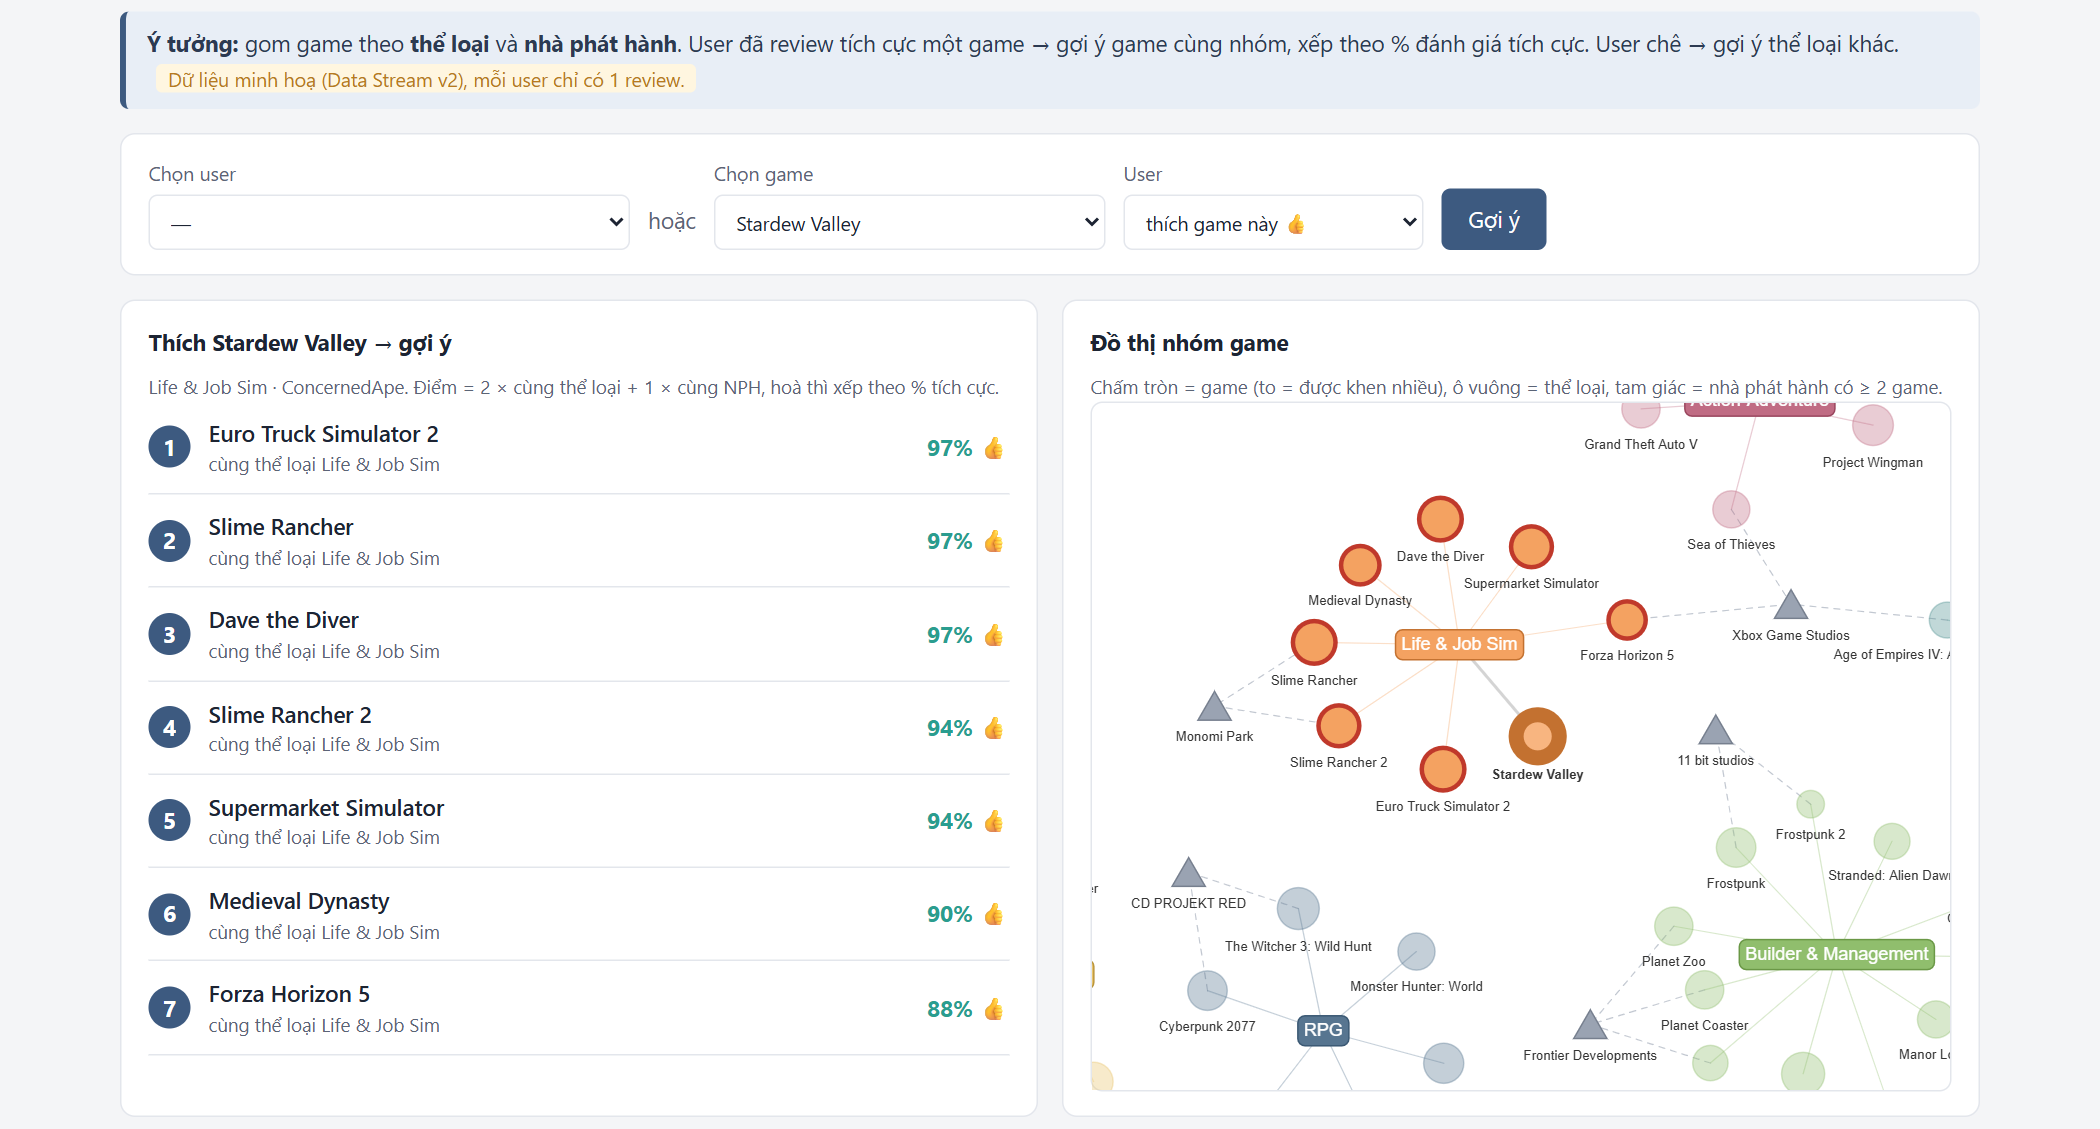
\includegraphics[width=0.88\textwidth]{app_reco.png}
    \caption{Recommendation page of the demo application (Vietnamese interface) for a user who liked Stardew Valley, with the genre/publisher graph.}
    \label{fig:appreco}
\end{figure}

\section{Discussion}

The results answer the instructor's question about deeper models with a nuanced picture. A pre-trained transformer gives a clear and statistically reliable improvement on every main metric (summarised in Table~\ref{tab:summary}); models trained from scratch on 7,000 reviews do not. Keywords are most useful as hints inside the transformer and when few labels are available. Where the transformer did not help, namely sentences with conflicting aspects, a likely cause is that each aspect's polarity depends on the clause structure of the sentence, which the model does not learn from a few hundred examples. Finally, part of the remaining sentiment errors comes from the verdicts rather than from the models, and these reviews are precisely what the suspicious review detector is designed to surface.
